\documentclass[twoside]{article}

% Packages required by doxygen
\usepackage{calc}
\usepackage{doxygen}
\usepackage{graphicx}
\usepackage[utf8]{inputenc}
\usepackage{makeidx}
\usepackage{multicol}
\usepackage{multirow}
\usepackage{textcomp}
\usepackage[table]{xcolor}

% Font selection
\usepackage[T1]{fontenc}
\usepackage{mathptmx}
\usepackage[scaled=.90]{helvet}
\usepackage{courier}
\usepackage{amssymb}
\usepackage{sectsty}
\renewcommand{\familydefault}{\sfdefault}
\allsectionsfont{%
  \fontseries{bc}\selectfont%
  \color{darkgray}%
}
\renewcommand{\DoxyLabelFont}{%
  \fontseries{bc}\selectfont%
  \color{darkgray}%
}

% Page & text layout
\usepackage{geometry}
\geometry{%
  a4paper,%
  top=2.5cm,%
  bottom=2.5cm,%
  left=2.5cm,%
  right=2.5cm%
}
\tolerance=750
\hfuzz=15pt
\hbadness=750
\setlength{\emergencystretch}{15pt}
\setlength{\parindent}{0cm}
\setlength{\parskip}{0.2cm}
\makeatletter
\renewcommand{\paragraph}{%
  \@startsection{paragraph}{4}{0ex}{-1.0ex}{1.0ex}{%
    \normalfont\normalsize\bfseries\SS@parafont%
  }%
}
\renewcommand{\subparagraph}{%
  \@startsection{subparagraph}{5}{0ex}{-1.0ex}{1.0ex}{%
    \normalfont\normalsize\bfseries\SS@subparafont%
  }%
}
\makeatother

% Headers & footers
\usepackage{fancyhdr}
\pagestyle{fancyplain}
\fancyhead[LE]{\fancyplain{}{\bfseries\thepage}}
\fancyhead[CE]{\fancyplain{}{}}
\fancyhead[RE]{\fancyplain{}{\bfseries\leftmark}}
\fancyhead[LO]{\fancyplain{}{\bfseries\rightmark}}
\fancyhead[CO]{\fancyplain{}{}}
\fancyhead[RO]{\fancyplain{}{\bfseries\thepage}}
\fancyfoot[LE]{\fancyplain{}{}}
\fancyfoot[CE]{\fancyplain{}{}}
\fancyfoot[RE]{\fancyplain{}{\bfseries\scriptsize Generated on Thu Mar 12 2015 08\-:08\-:14 for Zadanie 1 by Doxygen }}
\fancyfoot[LO]{\fancyplain{}{\bfseries\scriptsize Generated on Thu Mar 12 2015 08\-:08\-:14 for Zadanie 1 by Doxygen }}
\fancyfoot[CO]{\fancyplain{}{}}
\fancyfoot[RO]{\fancyplain{}{}}
\renewcommand{\footrulewidth}{0.4pt}
\renewcommand{\sectionmark}[1]{%
  \markright{\thesection\ #1}%
}

% Indices & bibliography
\usepackage{natbib}
\usepackage[titles]{tocloft}
\setcounter{tocdepth}{3}
\setcounter{secnumdepth}{5}
\makeindex

% Hyperlinks (required, but should be loaded last)
\usepackage{ifpdf}
\ifpdf
  \usepackage[pdftex,pagebackref=true]{hyperref}
\else
  \usepackage[ps2pdf,pagebackref=true]{hyperref}
\fi
\hypersetup{%
  colorlinks=true,%
  linkcolor=blue,%
  citecolor=blue,%
  unicode%
}

% Custom commands
\newcommand{\clearemptydoublepage}{%
  \newpage{\pagestyle{empty}\cleardoublepage}%
}


%===== C O N T E N T S =====

\begin{document}

% Titlepage & ToC
\hypersetup{pageanchor=false}
\pagenumbering{roman}
\begin{titlepage}
\vspace*{7cm}
\begin{center}%
{\Large Zadanie 1 }\\
\vspace*{1cm}
{\large Generated by Doxygen 1.8.6}\\
\vspace*{0.5cm}
{\small Thu Mar 12 2015 08:08:14}\\
\end{center}
\end{titlepage}
\tableofcontents
\pagenumbering{arabic}
\hypersetup{pageanchor=true}

%--- Begin generated contents ---
\section{Class Index}
\section{Class List}
Here are the classes, structs, unions and interfaces with brief descriptions\+:\begin{DoxyCompactList}
\item\contentsline{section}{\hyperlink{a00001}{Array\+Lista} \\*Klasa \hyperlink{a00001}{Array\+Lista} }{\pageref{a00001}}{}
\item\contentsline{section}{\hyperlink{a00002}{Benchmarker} \\*Klasa \hyperlink{a00002}{Benchmarker} }{\pageref{a00002}}{}
\item\contentsline{section}{\hyperlink{a00003}{Hasz\+Tab} \\*Klasa \hyperlink{a00003}{Hasz\+Tab} }{\pageref{a00003}}{}
\item\contentsline{section}{\hyperlink{a00004}{Kolejka} \\*Klasa \hyperlink{a00004}{Kolejka} }{\pageref{a00004}}{}
\item\contentsline{section}{\hyperlink{a00005}{Lista} \\*Klasa \hyperlink{a00005}{Lista} }{\pageref{a00005}}{}
\item\contentsline{section}{\hyperlink{a00006}{Stos} \\*Klasa \hyperlink{a00006}{Stos} }{\pageref{a00006}}{}
\end{DoxyCompactList}

\section{File Index}
\subsection{File List}
Here is a list of all files with brief descriptions\-:\begin{DoxyCompactList}
\item\contentsline{section}{\hyperlink{a00002}{Benchmark.\-cpp} \\*Metody klasy \hyperlink{a00001}{Benchmarker} }{\pageref{a00002}}{}
\item\contentsline{section}{\hyperlink{a00003}{Benchmark.\-hh} \\*Definicja klasy Benchmark }{\pageref{a00003}}{}
\item\contentsline{section}{\hyperlink{a00004}{main.\-cpp} \\*Modul glowny }{\pageref{a00004}}{}
\end{DoxyCompactList}

\section{Class Documentation}
\hypertarget{a00001}{\subsection{Benchmarker Class Reference}
\label{a00001}\index{Benchmarker@{Benchmarker}}
}


Klasa benchmarku.  




{\ttfamily \#include $<$Benchmark.\-hh$>$}

\subsubsection*{Public Member Functions}
\begin{DoxyCompactItemize}
\item 
\hyperlink{a00001_aab7e84d7ce96b1a26eee22f9fc11a55a}{Benchmarker} ()
\begin{DoxyCompactList}\small\item\em Konstruktor bezparametryczny . \end{DoxyCompactList}\item 
\hyperlink{a00001_a2ef2105cab075e03500d057780c7694e}{$\sim$\-Benchmarker} ()
\begin{DoxyCompactList}\small\item\em Destruktor bezparametryczny. \end{DoxyCompactList}\item 
long long int \hyperlink{a00001_af0281a2fc6e1cb2e0041d548f6163fee}{testuj} (int $\ast$, int $\ast$, int, int)
\begin{DoxyCompactList}\small\item\em Metoda przeprowadzajaca sprawdzenie czasy dzialania funkcji. sprawdzienie czasu dzialania mnozenia kazdego elementu tablicy razy 2. \end{DoxyCompactList}\item 
int $\ast$ \hyperlink{a00001_a917b8efeea3b8a82882be68e490548e8}{generuj\-\_\-dane} (int)
\end{DoxyCompactItemize}


\subsubsection{Detailed Description}
Klasa benchmarku. 

\subsubsection{Constructor \& Destructor Documentation}
\hypertarget{a00001_aab7e84d7ce96b1a26eee22f9fc11a55a}{\index{Benchmarker@{Benchmarker}!Benchmarker@{Benchmarker}}
\index{Benchmarker@{Benchmarker}!Benchmarker@{Benchmarker}}
\paragraph[{Benchmarker}]{\setlength{\rightskip}{0pt plus 5cm}Benchmarker\-::\-Benchmarker (
\begin{DoxyParamCaption}
{}
\end{DoxyParamCaption}
)}}\label{a00001_aab7e84d7ce96b1a26eee22f9fc11a55a}


Konstruktor bezparametryczny . 

\hypertarget{a00001_a2ef2105cab075e03500d057780c7694e}{\index{Benchmarker@{Benchmarker}!$\sim$\-Benchmarker@{$\sim$\-Benchmarker}}
\index{$\sim$\-Benchmarker@{$\sim$\-Benchmarker}!Benchmarker@{Benchmarker}}
\paragraph[{$\sim$\-Benchmarker}]{\setlength{\rightskip}{0pt plus 5cm}Benchmarker\-::$\sim$\-Benchmarker (
\begin{DoxyParamCaption}
{}
\end{DoxyParamCaption}
)}}\label{a00001_a2ef2105cab075e03500d057780c7694e}


Destruktor bezparametryczny. 



\subsubsection{Member Function Documentation}
\hypertarget{a00001_a917b8efeea3b8a82882be68e490548e8}{\index{Benchmarker@{Benchmarker}!generuj\-\_\-dane@{generuj\-\_\-dane}}
\index{generuj\-\_\-dane@{generuj\-\_\-dane}!Benchmarker@{Benchmarker}}
\paragraph[{generuj\-\_\-dane}]{\setlength{\rightskip}{0pt plus 5cm}int$\ast$ Benchmarker\-::generuj\-\_\-dane (
\begin{DoxyParamCaption}
\item[{int}]{}
\end{DoxyParamCaption}
)}}\label{a00001_a917b8efeea3b8a82882be68e490548e8}
\hypertarget{a00001_af0281a2fc6e1cb2e0041d548f6163fee}{\index{Benchmarker@{Benchmarker}!testuj@{testuj}}
\index{testuj@{testuj}!Benchmarker@{Benchmarker}}
\paragraph[{testuj}]{\setlength{\rightskip}{0pt plus 5cm}long long int Benchmarker\-::testuj (
\begin{DoxyParamCaption}
\item[{int $\ast$}]{tab, }
\item[{int $\ast$}]{dane, }
\item[{int}]{liczba\-\_\-przejsc, }
\item[{int}]{liczba\-\_\-danych}
\end{DoxyParamCaption}
)}}\label{a00001_af0281a2fc6e1cb2e0041d548f6163fee}


Metoda przeprowadzajaca sprawdzenie czasy dzialania funkcji. sprawdzienie czasu dzialania mnozenia kazdego elementu tablicy razy 2. 


\begin{DoxyParams}{Parameters}
{\em tab} & -\/ typu int$\ast$, wskaznik na tablice z wartosciami. \\
\hline
{\em dane} & -\/ typu int$\ast$, wskaznik na tablice z danymi generowanymi. \\
\hline
{\em liczba\-\_\-przejsc} & -\/ typu int, liczba przejsc przez dane. \\
\hline
{\em liczba\-\_\-danych} & -\/ typu int, liczba danych w tablicy. \\
\hline
\end{DoxyParams}
\begin{DoxyReturn}{Returns}
czas\-\_\-calkowity\-\_\-usredniony -\/ typu int, czas sredni dzialania funkcji. 
\end{DoxyReturn}


The documentation for this class was generated from the following files\-:\begin{DoxyCompactItemize}
\item 
\hyperlink{a00003}{Benchmark.\-hh}\item 
\hyperlink{a00002}{Benchmark.\-cpp}\end{DoxyCompactItemize}

\section{File Documentation}
\hypertarget{a00002}{}\section{Algorytm1 Class Reference}
\label{a00002}\index{Algorytm1@{Algorytm1}}


Klasa \hyperlink{a00002}{Algorytm1}.  




{\ttfamily \#include $<$Algorytm1.\+hh$>$}



Inheritance diagram for Algorytm1\+:
\nopagebreak
\begin{figure}[H]
\begin{center}
\leavevmode
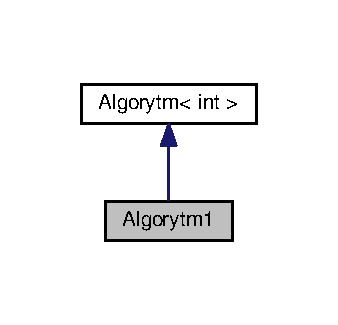
\includegraphics[width=162pt]{a00118}
\end{center}
\end{figure}


Collaboration diagram for Algorytm1\+:
\nopagebreak
\begin{figure}[H]
\begin{center}
\leavevmode
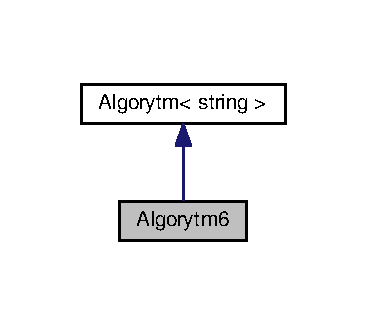
\includegraphics[width=162pt]{a00119}
\end{center}
\end{figure}
\subsection*{Public Member Functions}
\begin{DoxyCompactItemize}
\item 
\hyperlink{a00002_abb461ae4b741a82619039d789e0d2b0e}{$\sim$\+Algorytm1} ()
\item 
void \hyperlink{a00002_a0a9f86a1cf3b22e273042010d3a7d00f}{alokujdane} (\hyperlink{a00019}{Zasobnik}$<$ int $>$ $\ast$, int $\ast$, int)
\begin{DoxyCompactList}\small\item\em Metoda alokujaca na zasobniku dane. \end{DoxyCompactList}\item 
void \hyperlink{a00002_aca10f2c6923337e0ab928338e8989417}{wykonajalgorytm} (\hyperlink{a00019}{Zasobnik}$<$ int $>$ $\ast$, int $\ast$, int)
\begin{DoxyCompactList}\small\item\em Metoda wykonujaca konkretny algorytm. \end{DoxyCompactList}\end{DoxyCompactItemize}


\subsection{Detailed Description}
Klasa \hyperlink{a00002}{Algorytm1}. 

\subsection{Constructor \& Destructor Documentation}
\hypertarget{a00002_abb461ae4b741a82619039d789e0d2b0e}{}\index{Algorytm1@{Algorytm1}!````~Algorytm1@{$\sim$\+Algorytm1}}
\index{````~Algorytm1@{$\sim$\+Algorytm1}!Algorytm1@{Algorytm1}}
\subsubsection[{$\sim$\+Algorytm1}]{\setlength{\rightskip}{0pt plus 5cm}Algorytm1\+::$\sim$\+Algorytm1 (
\begin{DoxyParamCaption}
{}
\end{DoxyParamCaption}
)\hspace{0.3cm}{\ttfamily [inline]}}\label{a00002_abb461ae4b741a82619039d789e0d2b0e}


\subsection{Member Function Documentation}
\hypertarget{a00002_a0a9f86a1cf3b22e273042010d3a7d00f}{}\index{Algorytm1@{Algorytm1}!alokujdane@{alokujdane}}
\index{alokujdane@{alokujdane}!Algorytm1@{Algorytm1}}
\subsubsection[{alokujdane}]{\setlength{\rightskip}{0pt plus 5cm}void Algorytm1\+::alokujdane (
\begin{DoxyParamCaption}
\item[{{\bf Zasobnik}$<$ int $>$ $\ast$}]{Tab, }
\item[{int $\ast$}]{dane, }
\item[{int}]{liczba\+\_\+danych}
\end{DoxyParamCaption}
)\hspace{0.3cm}{\ttfamily [virtual]}}\label{a00002_a0a9f86a1cf3b22e273042010d3a7d00f}


Metoda alokujaca na zasobniku dane. 


\begin{DoxyParams}{Parameters}
{\em Tab} & -\/ typu Zasobnik$<$\+T$>$$\ast$, implementacja zasobnika \\
\hline
{\em dane} & -\/ typu T$\ast$, dane wygenerowane dla implementacji \\
\hline
{\em liczba\+\_\+danych} & -\/ typu int, liczba danych dla zasobnika \\
\hline
\end{DoxyParams}


Implements \hyperlink{a00001_a1e83fd87a20fd0a13ebbf1c81e457b61}{Algorytm$<$ int $>$}.

\hypertarget{a00002_aca10f2c6923337e0ab928338e8989417}{}\index{Algorytm1@{Algorytm1}!wykonajalgorytm@{wykonajalgorytm}}
\index{wykonajalgorytm@{wykonajalgorytm}!Algorytm1@{Algorytm1}}
\subsubsection[{wykonajalgorytm}]{\setlength{\rightskip}{0pt plus 5cm}void Algorytm1\+::wykonajalgorytm (
\begin{DoxyParamCaption}
\item[{{\bf Zasobnik}$<$ int $>$ $\ast$}]{Tab, }
\item[{int $\ast$}]{dane, }
\item[{int}]{liczba\+\_\+danych}
\end{DoxyParamCaption}
)\hspace{0.3cm}{\ttfamily [virtual]}}\label{a00002_aca10f2c6923337e0ab928338e8989417}


Metoda wykonujaca konkretny algorytm. 


\begin{DoxyParams}{Parameters}
{\em Tab} & -\/ typu Zasobnik$<$\+T$>$$\ast$, implementacja zasobnika \\
\hline
{\em dane} & -\/ typu T$\ast$, dane wygenerowane dla implementacji \\
\hline
{\em liczba\+\_\+danych} & -\/ typu int, liczba danych dla zasobnika \\
\hline
\end{DoxyParams}


Implements \hyperlink{a00001_ae97a52b1a728be1a819c9e9815f424e7}{Algorytm$<$ int $>$}.



The documentation for this class was generated from the following files\+:\begin{DoxyCompactItemize}
\item 
\hyperlink{a00021}{Algorytm1.\+hh}\item 
\hyperlink{a00020}{Algorytm1.\+cpp}\end{DoxyCompactItemize}

\hypertarget{a00003}{}\section{Kolejka Class Reference}
\label{a00003}\index{Kolejka@{Kolejka}}


Klasa \hyperlink{a00003}{Kolejka}.  




{\ttfamily \#include $<$Kolejka.\+hh$>$}

\subsection*{Public Member Functions}
\begin{DoxyCompactItemize}
\item 
\hyperlink{a00003_a37c886fdc73dce62b04da0381dec5484}{Kolejka} ()
\begin{DoxyCompactList}\small\item\em Konstruktor bezparametryczny. Konstruktor inicjalizujacy straznika\+\_\+poczatek i straznika\+\_\+koniec kolejki wartosciami N\+U\+L\+L , oraz rozmiar kolejki wartoscia 0. \end{DoxyCompactList}\item 
\hyperlink{a00003_a352f86ff08cd47be6c35c60bb0f873a6}{$\sim$\+Kolejka} ()
\begin{DoxyCompactList}\small\item\em Destruktor bezparametryczny kolejki. \end{DoxyCompactList}\item 
void \hyperlink{a00003_abdd1c95eb88905167ec26658b6b76611}{push} (int)
\begin{DoxyCompactList}\small\item\em Metoda umieszczajaca element na koncu kolejki. Metoda inkrementuje rozmiar podczas umieszczania elementu w kolejce. \end{DoxyCompactList}\item 
int \hyperlink{a00003_aa99d7c7459116c2331b301637b45b666}{pop} ()
\begin{DoxyCompactList}\small\item\em Metoda zdejmujaca element z poczatku kolejki. Metoda dekrementuje rozmiar przy zdejmowaniu elementu. \end{DoxyCompactList}\item 
int \hyperlink{a00003_a82920d7b90e967a4d5e175a20fe6de68}{size} ()
\begin{DoxyCompactList}\small\item\em Metoda zwracajaca wielkosc kolejki. \end{DoxyCompactList}\end{DoxyCompactItemize}


\subsection{Detailed Description}
Klasa \hyperlink{a00003}{Kolejka}. 

\subsection{Constructor \& Destructor Documentation}
\hypertarget{a00003_a37c886fdc73dce62b04da0381dec5484}{}\index{Kolejka@{Kolejka}!Kolejka@{Kolejka}}
\index{Kolejka@{Kolejka}!Kolejka@{Kolejka}}
\subsubsection[{Kolejka}]{\setlength{\rightskip}{0pt plus 5cm}Kolejka\+::\+Kolejka (
\begin{DoxyParamCaption}
{}
\end{DoxyParamCaption}
)}\label{a00003_a37c886fdc73dce62b04da0381dec5484}


Konstruktor bezparametryczny. Konstruktor inicjalizujacy straznika\+\_\+poczatek i straznika\+\_\+koniec kolejki wartosciami N\+U\+L\+L , oraz rozmiar kolejki wartoscia 0. 

\hypertarget{a00003_a352f86ff08cd47be6c35c60bb0f873a6}{}\index{Kolejka@{Kolejka}!````~Kolejka@{$\sim$\+Kolejka}}
\index{````~Kolejka@{$\sim$\+Kolejka}!Kolejka@{Kolejka}}
\subsubsection[{$\sim$\+Kolejka}]{\setlength{\rightskip}{0pt plus 5cm}Kolejka\+::$\sim$\+Kolejka (
\begin{DoxyParamCaption}
{}
\end{DoxyParamCaption}
)}\label{a00003_a352f86ff08cd47be6c35c60bb0f873a6}


Destruktor bezparametryczny kolejki. 



\subsection{Member Function Documentation}
\hypertarget{a00003_aa99d7c7459116c2331b301637b45b666}{}\index{Kolejka@{Kolejka}!pop@{pop}}
\index{pop@{pop}!Kolejka@{Kolejka}}
\subsubsection[{pop}]{\setlength{\rightskip}{0pt plus 5cm}int Kolejka\+::pop (
\begin{DoxyParamCaption}
{}
\end{DoxyParamCaption}
)}\label{a00003_aa99d7c7459116c2331b301637b45b666}


Metoda zdejmujaca element z poczatku kolejki. Metoda dekrementuje rozmiar przy zdejmowaniu elementu. 

\begin{DoxyReturn}{Returns}
wartosc -\/ typu int, wartosc zdejmowana z kolejki. 
\end{DoxyReturn}
\hypertarget{a00003_abdd1c95eb88905167ec26658b6b76611}{}\index{Kolejka@{Kolejka}!push@{push}}
\index{push@{push}!Kolejka@{Kolejka}}
\subsubsection[{push}]{\setlength{\rightskip}{0pt plus 5cm}void Kolejka\+::push (
\begin{DoxyParamCaption}
\item[{int}]{wartosc}
\end{DoxyParamCaption}
)}\label{a00003_abdd1c95eb88905167ec26658b6b76611}


Metoda umieszczajaca element na koncu kolejki. Metoda inkrementuje rozmiar podczas umieszczania elementu w kolejce. 


\begin{DoxyParams}{Parameters}
{\em wartosc} & -\/ typu int, wartosc umieszczana na koncu kolejki. \\
\hline
\end{DoxyParams}
\hypertarget{a00003_a82920d7b90e967a4d5e175a20fe6de68}{}\index{Kolejka@{Kolejka}!size@{size}}
\index{size@{size}!Kolejka@{Kolejka}}
\subsubsection[{size}]{\setlength{\rightskip}{0pt plus 5cm}int Kolejka\+::size (
\begin{DoxyParamCaption}
{}
\end{DoxyParamCaption}
)}\label{a00003_a82920d7b90e967a4d5e175a20fe6de68}


Metoda zwracajaca wielkosc kolejki. 

\begin{DoxyReturn}{Returns}
rozmiar -\/ typu int,rozmiar kolejki. 
\end{DoxyReturn}


The documentation for this class was generated from the following files\+:\begin{DoxyCompactItemize}
\item 
\hyperlink{a00011}{Kolejka.\+hh}\item 
\hyperlink{a00010}{Kolejka.\+cpp}\end{DoxyCompactItemize}

\hypertarget{a00004}{\subsection{main.\-cpp File Reference}
\label{a00004}\index{main.\-cpp@{main.\-cpp}}
}


Modul glowny.  


{\ttfamily \#include $<$cstdlib$>$}\\*
{\ttfamily \#include $<$iostream$>$}\\*
{\ttfamily \#include $<$fstream$>$}\\*
{\ttfamily \#include \char`\"{}Benchmark.\-hh\char`\"{}}\\*
Include dependency graph for main.\-cpp\-:
\nopagebreak
\begin{figure}[H]
\begin{center}
\leavevmode
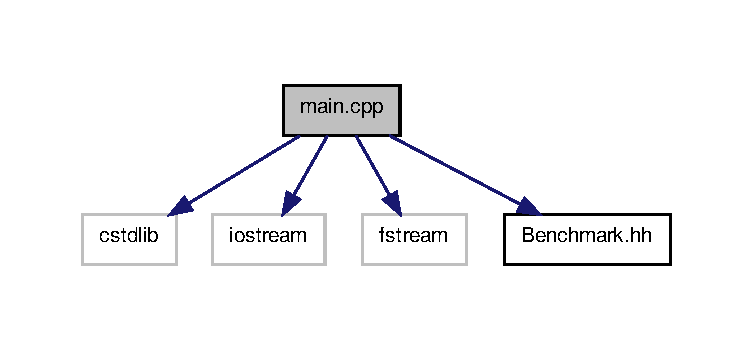
\includegraphics[width=350pt]{a00009}
\end{center}
\end{figure}
\subsubsection*{Functions}
\begin{DoxyCompactItemize}
\item 
int \hyperlink{a00004_ae66f6b31b5ad750f1fe042a706a4e3d4}{main} ()
\begin{DoxyCompactList}\small\item\em Funkcja glowna programu. \end{DoxyCompactList}\end{DoxyCompactItemize}


\subsubsection{Detailed Description}
Modul glowny. Plik zawiera funkcje main. 

\subsubsection{Function Documentation}
\hypertarget{a00004_ae66f6b31b5ad750f1fe042a706a4e3d4}{\index{main.\-cpp@{main.\-cpp}!main@{main}}
\index{main@{main}!main.cpp@{main.\-cpp}}
\paragraph[{main}]{\setlength{\rightskip}{0pt plus 5cm}int main (
\begin{DoxyParamCaption}
{}
\end{DoxyParamCaption}
)}}\label{a00004_ae66f6b31b5ad750f1fe042a706a4e3d4}


Funkcja glowna programu. 



Here is the call graph for this function\-:
\nopagebreak
\begin{figure}[H]
\begin{center}
\leavevmode
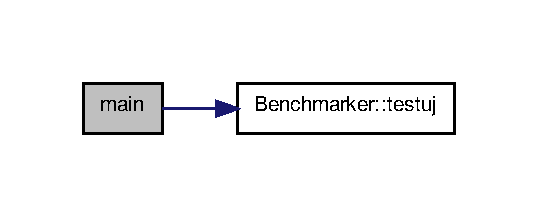
\includegraphics[width=258pt]{a00004_ae66f6b31b5ad750f1fe042a706a4e3d4_cgraph}
\end{center}
\end{figure}



%--- End generated contents ---

% Index
\newpage
\phantomsection
\addcontentsline{toc}{section}{Index}
\printindex

\end{document}
